\documentclass{article}
\usepackage{tikz}
\usetikzlibrary{arrows.meta}

\begin{document}

\begin{figure}[h]
    \centering
    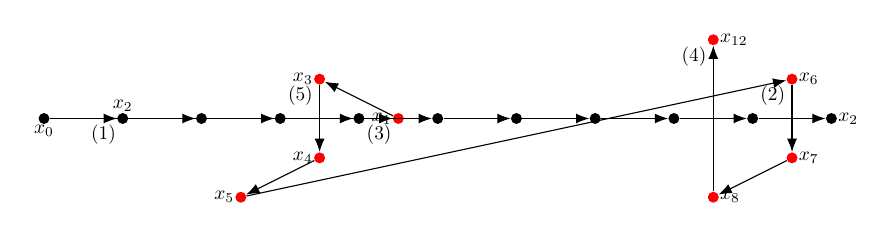
\begin{tikzpicture}[scale=0.5, every node/.style={scale=0.7}]
        % Define the nodes
        \node[fill,circle,inner sep=2pt] (u) at (-10,0) {};
        \node[fill,circle,inner sep=2pt] (v) at (-8,0) {};
        \node[fill,circle,inner sep=2pt] (w) at (-6,0) {};
        \node[fill,circle,inner sep=2pt] (x) at (-4,0) {};
        \node[fill,circle,inner sep=2pt] (y) at (-2,0) {};
        \node[fill,circle,inner sep=2pt] (z) at (0,0) {};
        \node[fill,circle,inner sep=2pt] (a) at (2,0) {};
        \node[fill,circle,inner sep=2pt] (b) at (4,0) {};
        \node[fill,circle,inner sep=2pt] (c) at (6,0) {};
        \node[fill,circle,inner sep=2pt] (d) at (8,0) {};
        \node[fill,circle,inner sep=2pt] (e) at (10,0) {};

        \node[fill,red,circle,inner sep=2pt] (x1) at (-1,0) {};
        \node[fill,red,circle,inner sep=2pt] (x2) at (-3,1) {};
        \node[fill,red,circle,inner sep=2pt] (x3) at (-3,-1) {};
        \node[fill,red,circle,inner sep=2pt] (x4) at (-5,-2) {};
        \node[fill,red,circle,inner sep=2pt] (x5) at (9,1) {};
        \node[fill,red,circle,inner sep=2pt] (x6) at (9,-1) {};
        \node[fill,red,circle,inner sep=2pt] (x7) at (7,-2) {};
        \node[fill,red,circle,inner sep=2pt] (x8) at (7,2) {};

        \foreach \from/\to in {u/v,v/w,w/x,x/y,y/z,z/a,a/b,b/c,c/d,d/e,u/x1,x1/x2,x2/x3,x3/x4,x4/x5,x5/x6,x6/x7,x7/x8}
            \draw[-Latex] (\from) -- (\to);

        % Labels
        \node[below] at (u) {$x_0$};
        \node[left] at (-1,0) {$x_1$};
        \node[right] at (10,0) {$x_2$};
        \node[above] at (v) {$x_2$};
        \node[left] at (-3,1) {$x_3$};
        \node[left] at (-3,-1) {$x_4$};
        \node[left] at (-5,-2) {$x_5$};
        \node[right] at (9,1) {$x_6$};
        \node[right] at (9,-1) {$x_7$};
        \node[right] at (7,-2) {$x_8$};
        \node[right] at (7,2) {$x_{12}$};
        
        % Subscript labels
        \node[below left] at (v) {(1)};
        \node[below left] at (x5) {(2)};
        \node[below left] at (x1) {(3)};
        \node[below left] at (x8) {(4)};
        \node[below left] at (x2) {(5)};
    \end{tikzpicture}
    \caption{Illustration of trees $T_i$ and their corresponding red vertices set $S_i$.}
\end{figure}

\end{document}